\documentclass[10pt]{bmc_article}

\usepackage{a4wide}  % Formatting web addresses  
\usepackage{url}  % Formatting web addresses  
\usepackage{ifthen}  % Conditional 
\usepackage{multicol}   %Columns
\usepackage[utf8]{inputenc} %unicode support
\urlstyle{rm}
\usepackage{cite}
\usepackage{graphicx}

\newboolean{publ}

%Review style settings
\newenvironment{bmcformat}{\begin{raggedright}\baselineskip20pt\sloppy\setboolean{publ}{false}}{\end{raggedright}\baselineskip20pt\sloppy}
%Publication style settings
%\newenvironment{bmcformat}{\fussy\setboolean{publ}{true}}{\fussy}

\begin{document}
\begin{bmcformat}

%\pretitle{}
\title{The ChEMBL database as Linked Open Data}
 
\author{Egon~L.~Willighagen$^{1,*}$\email{Egon~L.~Willighagen - egon.willighagen@maastrichtuniversity.nl, \url{http://twitter.com/egonwillighagen}}\and
Andra~Waagmeester$^1$\email{Andra Waagmeester - andra.waagmeester@maastrichtuniversity.nl, \url{http://twitter.com/andrawaag}}\and
Ola Spjuth$^2$\email{Ola Spjuth - ola.spjuth@farmbio.uu.se}\and
Peter~Ansell$^3$\email{Peter Ansell - p\_ansell@yahoo.com, \url{http://twitter.com/p_ansell}}\and
Antony~J.~Williams$^4$\email{Antony J. Williams - WilliamsA@rsc.org, \url{http://twitter.com/ChemConnector}}\and
Valery~Tkachenko$^4$\email{Valery Tkachenko - TkachenkoV@rsc.org}\and
Janna~Hastings$^5$\email{Janna Hastings - hastings@ebi.ac.uk}\and
Mark~Davies$^6$\email{Mark Davies - mdavies@ebi.ac.uk, \url{http://twitter.com/mdavies12}}\and
John~P.~Overington$^6$\email{John P. Overington - jpo@ebi.ac.uk}\and
Anna~Gaulton$^6$\email{Anna Gaulton - agaulton@ebi.ac.uk}\and
Bin~Chen$^7$\email{Bin Chen - binchen@indiana.edu, \url{http://twitter.com/binchenindiana}}\and
David~J.~Wild$^7$\email{David J. Wild - djwild@indiana.edu, \url{http://twitter.com/davidjohnwild}}
}

\address{\iid(1)Department of Bioinformatics - BiGCaT, Maastricht University, P.O. Box 616, UNS50 Box 19, NL-6200 MD, Maastricht, The Netherlands  \\
\iid(2)Department of Pharmaceutical Biosciences, Uppsala University, PO Box 591, SE-751 24, Uppsala, Sweden \\
\iid(3)University of Queensland, St Lucia, Qld 4072, Australia \\
\iid(4)Royal Society of Chemistry, 904 Tamaras Circle, Wake Forest, NC 27587, U.S.A. \\
\iid(5)Cheminformatics and Metabolism, European Bioinformatics Institute, Wellcome Trust Genome Campus, Hinxton, Cambridgeshire, CB10 1SD, United Kingdom \\
\iid(6)Chemogenomics, European Bioinformatics Institute, Wellcome Trust Genome Campus, Hinxton, Cambridgeshire, CB10 1SD, United Kingdom \\ 
\iid(7)School of Informatics and Computing, Indiana University, Bloomington, IN, U.S.A.
}

\maketitle

\begin{abstract}
\paragraph*{Background:}
Making data available as Linked Data using Resource Description Framework (RDF) promotes integration with other web resources.
RDF documents can natively link to related data, and others can link back using Universal Resource Identifiers (URIs).
RDF makes the data machine-readable and uses extensible vocabularies for additional information, making it easier
to scale up inference and data analysis.
\paragraph*{Results:}
This paper describes recent developments in an ongoing project converting data from the ChEMBL database into RDF triples.
Relative to earlier versions, this updated version of ChEMBL-RDF uses recently introduced ontologies, including CHEMINF and CiTO;
exposes more information from the database; and is now available as dereferencable, linked data.
To demonstrate these new features, we present novel use cases showing further integration with
other web resources, including Bio2RDF, Chem2Bio2RDF, and ChemSpider, and showing the use of standard
ontologies for querying.
\paragraph*{Conclusions:}
We have illustrated the advantage of using open standards and ontologies to link the ChEMBL database
to other databases. Using those links and the knowledge encoded in standards and ontologies, the ChEMBL-RDF
resource creates a foundation for integrated semantic web cheminformatics applications, 
such as the presented decision support.
\end{abstract}


%%%%%%%%%%% The article body starts:

\section*{Introduction}
\label{s1}


The current scientific data deluge, in which datasets grow faster in size and complexity than scientists can keep up with,
defines several new challenges for information systems. Scientists wish to 
discover new, unique, and significant patterns in datasets that explain biological 
phenomena not yet understood. The discovery of new patterns showing the 
causes and effects of various biological phenomena is often beyond the scope of single datasets.
For example, systems biologists integrate micro-array differential expression datasets to 
biological pathways, using various other datasets to provide evidence for the links~\cite{Staab2007}. 
Another prominent example is drug discovery, in which a new unique chemical entity is designed or discovered 
based on descriptions of its required biological properties. This process requires the effective 
linkage of many scientific datasets that are both sparse and are growing independently from each
other~\cite{Belleau2008,Samwald2011,Williams2012}.

ChEMBL contains descriptions for biological activities involving over a million chemical 
entities, extracted primarily from scientific literature. This provides a unique resource for drug researchers~\cite{Gaulton2012,Warr2009}.
It is updated on a fairly frequent basis as the existing data is further curated and new data is added. 
The ChEMBL dataset is available for download and can be browsed using a web interface and web services.
The former requires scientists to import the data into a relational database, while the 
latter limits the machine access to the data. ChEMBL also provides web services for programmatic
access, but these are limited to the specific types of queries which are encoded in the web service API. 

Using the right to download, modify, and redistribute the ChEMBL data, two independent teams
have previously mapped the ChEMBL relational database to the Resource Description Framework (RDF), resulting
in Chem2Bio2RDF~\cite{Chen2010} and ChEMBL-RDF~\cite{Willighagen2011}. RDF is a framework where
knowledge is represented by small so-called triples, reflecting ``facts''. A fact can
be given on any topic, and RDF therefore talks about \textit{things} very generically~\cite{Miller:04:RP}. Things in RDF
are represented by resources named with Universal Resource Identifiers (URI). When the URI can be resolved, 
for example using the HTTP protocol, it creates \emph{linked data}~\cite{Bizer2008}. RDF is
developed as an open standard by the World Wide Web Consortium, and provides a knowledge
representation framework that applies to many, if not all, domains, making it a successful 
approach to data integration in the life sciences.

This paper presents an update on the ChEMBL-RDF data set, including details of the latest structures
and ontologies used to map ChEMBL to RDF, along with new use cases, showing 
links to other datasets using their RDF URIs to further support research in the life sciences.

\section*{Methods}
\label{s2}

The ChEMBL version used in this paper is ChEMBL 13, which was released on 29 February 2012.
The SQL data dump provided by ChEMBL was inserted into a local MySQL database. A set of SQL queries 
were then executed to generate RDF triples using a set of PHP scripts. The scripts use SQL to
query the database and output triples using print statements. Custom PHP scripts have been used
as a light-weight soluton to provide a Linked Data API via a Apache webserver, as well as to
create data files with triples. These scripts are Open Source 
and are available from the source code hosting service, GitHub~\cite{ChEMBLRDFGitHub}. This process 
has been outlined in a best practices note by the W3C Health Care and Life Sciences Interest
Group~\cite{Marshall2012}. This process has not changed much since its original description.

However, the previous ChEMBL-RDF conversion used custom predicates and classes to represent RDF triples, defining
an ad-hoc ontology~\cite{Willighagen2011}. The current version, instead, uses community-proposed
ontologies, making the RDF more interoperable with the RDF offerings of different databases. 
The new triple dataset uses standard ontologies
including the Bibliography Ontology~\cite{Giasson2011} and the Citation Typing Ontology (CiTO)~\cite{Shotton2010} for literature
references and citations, and domain ontologies such the Protein Ontology\cite{Sidhu2006} and the Chemical Information
Ontology\cite{Hastings2011}. Throughout this paper various prefixes are used to denote different ontology 
namespaces to simplify the RDF examples. These prefixes are outlined in Table~\ref{namespaces}.

To expose the ChEMBL-RDF data two approaches have been adopted. First, a SPARQL end point is being
hosted at Uppsala University, using the Open-Source Edition of the Virtuoso software~\cite{Virtuoso}. Usage is free, but the
allowed volume of querying is capped, based on the estimated computational effort. Second, resources have
been made dereferencable via the \url{http://linkedchemistry.info} resource. The Kasabi
platform~\cite{kasabi} was used for a period of time, until that project was discontinued.
The Uppsala SPARQL end point still uses resource URIs based on the Kasabi approach, following a similar
URI pattern where linkedchemistry.info/chembl is replaced by data.kasabi.com/dataset/chembl-rdf.

Although many parts of the ChEMBL-RDF 13 dataset now use community based ontologies, some 
terms from the previous ad-hoc ontology are still used because no community alternative is yet available. 
These terms were created under the 
URI namespace \textit{http://rdf.farmbio.uu.se/chembl/onto/\#}, and are referenced here using the
prefix: \textit{chembl}.

%As a method to further test the access and possibilities of this Linked Data version of
%ChEMBL,  new uses cases have been developed for this paper.

\section*{Results}
\label{s3}

We present here the updated ChEMBL-RDF, including a description of the mapping process 
and the identification of links to other datasets. Because the primary purpose of of this
paper is to expose the ChEMBL data as linked data, less focus has been placed on ontologically
capturing the fine details of the pharmacological literature. This is the reason why
many concepts are not mapped to existing ontologies, though also the lack of ontologies
with a clear open license restrict the options.

\subsection*{Data Structure}

For each of the common resource classes, a triple pattern was defined, following the
data available in the relational database. Unless the ontological meaning of the data
in the database was very clear, the classes are annotated with concepts as implicitly
defined by the relational database. For example, the activity concept in the triples
merely follows the activity table in the database. As such, the concept of chembl:Activity
is implied by the content of that table in the relational database.

However, where the database content is well-defined, specific ontologies have been used.
For example, where the database specifies literature from which data was extraced,
the CiTO ontology is used. The choice of the ontologies is driven by the use cases and
compatibility with other Linked Data projects, rather than formal ontological arguments.
We have not observed ontological contradictions based on these choices.

Figure~\ref{f1} shows how the various resource classes are linked together, detailed in
this section at a triple level.
The core concept in the ChEMBL database is that of the biological activity.
While ChEMBL provides both the original activities as found in literature
and standardized values allowing comparison between studies, the triples only
make the latter available. The links to the literature are encoded using the CiTO ontology.
This results in a set of triples that look like:

\begin{small}
\begin{verbatim}
act:a31863
 a       chembl:Activity ;
 cito:citesAsDataSource
  res:r6424 ;
 chembl:forMolecule mol:m180094 ;
 chembl:onAssay assay:a54505 ;
 chembl:relation ">" ;
 chembl:standardUnits
  "nM" ;
 chembl:standardValue
  "100000"^^xsd:float ;
 chembl:type "IC50" .
\end{verbatim}
\end{small}

More than five thousand different activity types, represented by the chembl:type predicate,
are captured by the ChEMBL database.
The top five types are ``Potency'' (43\%), ``IC50'' (13\%), ``MIC'' (4.6\%), ``Inhibition'' (3.7\%),
and ``Ki'' (3.6\%). The activity types in ChEMBL-RDF are currently not available as, or
linked to, an ontology. The BioAssay Ontology could be a future option~\cite{Visser2011}.

The activities themselves are measured against assays, which make up a second important
resource type. Various assay types are found in the database: \verb+chembl:ADMET+, \verb+chembl:Binding+,
\verb+chembl:Functional+, \verb+chembl:Property+, and \verb+chembl:Unassigned+.

\begin{small}
\begin{verbatim}
assay:a17
 a chembl:Assay ;
 cito:citesAsDataSource
  res:r11347 ;
 chembl:hasAssayType chembl:ADMET ;
 chembl:hasDescription
  "Inhibition of ... hydroxylase" .
\end{verbatim}
\end{small}

Each assay measures activities against one or more particular biological targets. To each
target the ChEMBL database associates a confidence score (see the Compound Selectivity
example). Because this score is specific
for each target, the following construct is used:

\begin{small}
\begin{verbatim}
assay:a17 chembl:hasTargetScore assay:a17/score/t100122 .
assay:a17/score/t100122
 chembl:forTarget target:t100122 ;
 chembl:hasConfScore "7"^^xsd:int .  
\end{verbatim}
\end{small}

The ChEMBL database
recognizes various target types: \verb+pro:PR_0000001+, \verb+chembl:ADMET+, \verb+chembl:CELL-LINE+,
\verb+chembl:NUCLEIC-ACID+, \verb+chembl:ORGANISM+, \verb+chembl:SUBCELLULAR+, \verb+chembl:TISSUE+,
\verb+chembl:UNCHECKED+, and \verb+chembl:UNKNOWN+. The latter two are currently defined as
explicit types, thus effectively implementing a closed-world approach. 

A target specification can then look like:

\begin{small}
\begin{verbatim}
target:t1
 a chembl:Target ;
 rdfs:subClassOf pro:PR_000000001 ;
 rdfs:label "Glucoamylase" , 
  "Maltase-glucoamylase, intestinal" ;
 dc:identifier "uniprot:O43451" ,
   "3.2.1.3" ;
 dc:title "Maltase-glucoamylase" ;
 chembl:classL1 "Enzyme" ;
 chembl:hasDescription
  "Maltase-glucoamylase, intestinal" ;
 chembl:hasKeyword "Glycosidase" , 
  "Membrane" , "Sulfation" ;
 chembl:organism "Homo sapiens" .
\end{verbatim}
\end{small}

For drug discovery, the drug-like compounds themselves are the main topic of study.
ChEMBL contains many different compound types, mostly small molecules,
but also peptides, proteins, antibodies, oligosaccharides, oligonucleotides, and
even cells. ChEMBL-RDF follows the approach used by the CHEMINF ontology,
and encodes drugs as classes, rather than instances, and they subclass
other classes defined by several ontologies for these types. For example, protein drugs subclass the
Protein class from the PRotein Ontology (PR\_000000001), instead that these drugs are
of the Protein type. Each drug is a class itself. Likewise, small
molecules subclass the Chemical Entity class from the CHEMINF
ontology (CHEMINF\_000000) (which is itself equivalent to the Chemical Entity class in ChEBI, CHEBI\_24431), 
and oligosaccharides and oligonucleotides
subclass their respective matches in the CHEBI ontology (CHEBI\_50699
and CHEBI\_7754). To ensure we can look up all entities for which activities
are reported, we subclass everything from the BFO 1.1 class MaterialEntity~\cite{Smith2004},
which is a superclass of the CHEMINF Chemical Entity class.

It should also be noted that all drug-like entities in ChEMBL are not ontologically
subclassing a drug class. Instead, we give the entities the role of drug: only within a
particular context, they would be drug. If not used as medication, they are not drug.
Moreover, the triples only attach this drug role to approved drugs, as defined by the
ChEMBL database. All drug-like entities in the database do not have the role of drug.
The role is triplified using the OBO and ChEBI ontologies in the following manner,
where CHEBI\_23888 is the ontological entry for ``drug role'' in ChEBI:

\begin{small}
\begin{verbatim}
mol:m4 obo:has_role chebi:CHEBI_23888 .
\end{verbatim}
\end{small}

The name and synonyms for each drug are
provided as labels. If SMILES, InChI, or InChIKeys are given for a drug, then these are
provided via the CHEMINF formalism.
The CHEMINF ontology has been used here because of it's flexibility in defining
descriptor types and their origin and meaning. By allowing an ontology of descriptors,
we enable comparing values between databases semantically. Differences in, for example,
the SMILES may then be explained by the software used for that descriptor.

Example output for ChEMBL406142 looks like:

\begin{small}
\begin{verbatim}
mol:m41
 rdfs:label "ChEMBL406142" , 
   "Bis(3-[1 .... yl]-propionamide)" ;
 rdfs:subClassOf bfo:MaterialEntity ;
 rdfs:subClassOf cheminf:CHEMINF_000000 ;
 cheminf:CHEMINF_000200
  m41:inchikey , m41:smiles , m41:inchi .

m41:inchikey
 a cheminf:CHEMINF_000059 ;
 cheminf:SIO_000300
   "LMCOMIDLRGMFCZ-RIPOXUOASA-N" .

m41:smiles
 a cheminf:CHEMINF_000018 ;
 cheminf:SIO_000300
  "CC(C)C[C@@H]1N2C= .... O)C7=O)NC1=O)C2=O" .

m41:inchi
 a cheminf:CHEMINF_000113 ;
 cheminf:SIO_000300
  "InChI=1S/C82H102N .... 66+,67+,68+/m1/s1" .

chemblid:ChEMBL406142
 owl:equivalentClass mol:m41 .
\end{verbatim}
\end{small}

Similarly, properties of small molecules are available from ChEMBL, and as of ChEMBL-RDF 13
these too are exposed in triple format. Like the InChI and InChIKey, these are provided using the
CHEMINF ontology. Here is, for example, the logP value (as distributed with ChEMBL and
calculated with ACD/Labs software):

\begin{small}
\begin{verbatim}
mol:m1
 cheminf:CHEMINF_000200 m1:alogp .

m1:alogp
 a cheminf:CHEMINF_000305 ;
 cheminf:SIO_000300
  "3.344"^^xsd:double .
\end{verbatim}
\end{small}

The literature from which all this data was extracted, is replicated from the database,
but only a subset of the possible information about that literature is provided. In all cases 
the PubMed Identifiers (PMIDs) and Digital Object Identifiers (DOIs) are used to link
to authoritative database, as outlined later in this paper.
The properties are provided using the BIBO ontology, which is an open sourced ontology
for bibliographic information, compatible with the CiTO ontology:

\begin{small}
\begin{verbatim}
res:r1
 a bibo:Article ;
 dc:date "2004" ;
 dc:isPartOf
  journal:j6c706049c2e08871b7c46a6528065736 ;
 bibo:issue "1" ;
 bibo:pageEnd "9" ;
 bibo:pageStart "1" ;
 bibo:pmid "14695813" ;
 bibo:volume "47" .

journal:j6c706049c2e08871b7c46a6528065736
 a bibo:Journal ;
 dc:title "J. Med. Chem." .
\end{verbatim}
\end{small}

\subsection*{Data Statistics and Validation}

Each release of the ChEMBL database is accompanied by a set of release statistics, which help 
provide a concise content overview of the release in question. The ChEMBL 13 release counts
are as follows:
\begin{itemize}
  \item 8,845 targets
  \item 1,143,682 distinct molecules
  \item 6,933,068 activities
  \item 617,681 assays
  \item 44,682 documents
\end{itemize}

These counts are important as firstly they show continued growth in ChEMBL data, as seen 
in all previous releases. Secondly, these counts can help validate any transformations, 
which have been applied to the relational data model traditionally used to store the ChEMBL 
data.  The following SPARQL queries attempt to provide a high level validation of the 
ChEMBL-RDF by regenerating the ChEMBL 13 release statistics.

The following SPARQL query returns 8,845 ChEMBL targets:
     
\begin{small}
\begin{verbatim}
select count(*) WHERE {
  ?s ?p chembl:Target .
}
\end{verbatim}
\end{small}

A similar SPARQL query, replacing \verb+chembl:Target+ with \verb+bfo:MaterialEntity+, returns 1,143,682 entities for which activities are captured in ChEMBL, and by using \verb+chembl:Assay+, the query returns the total of 617,681 ChEMBL assays.
It should be noted that last query returns five entries less than the SQL database, because the
triple generation requires the assay type to be defined, which is not the case for those 
five assays. With \verb+chembl:Activity+ and \verb+bibo:Article+, we count 6,933,068 ChEMBL activities and 44,681 documents,
respectively. The document count is one fewer than appears 
in the ChEMBL 13 release notes~\cite{ChEMBL13ReleaseNotes}, as the result does not include the doc\_id -1, as this refers to the 
unpublished dataset, not itself a valid \verb+bibo:Article+.

Reproduction of the ChEMBL release statistics through querying ChEMBL-RDF with SPARQL 
provides end users with a high degree of confidence that the ChEMBL-RDF contains the same 
core content as the source relational database. The development of a validation test suite
is being discussed but not yet implemented; testing criteria other then the here presented
summarizing counts would change with each release due to curation events. Interactive,
manual curation of the conversion process as employed by the authors already is more effective
at this moment.

\subsection*{Linked Open Data}

To integrate ChEMBL-RDF with RDF versions of other scientific datasets, we link out to various resources.
These links are shown in Figure~\ref{2}. Triples for compounds link out to ChemSpider 
using the complementary index and OpenMolecules RDF using InChI values~\cite{Pence2010,Bradley2009,Willighagen2011}.
Protein links are given to Bio2RDF~\cite{Belleau2008}
using the UniProt identifier~\cite{TheUniProtConsortium2010}. Literature references are directed to CrossRef and Bio2RDF 
using the DOIs and PubMed identifiers, respectively~\cite{Bilder2011}.

The predicates used to capture the links to these databases are
\verb+rdfs:seeAlso+, \verb+skos:exactMatch+, \verb+owl:equivalentClass+, and \verb+owl:sameAs+. 
These relations are ordered according to their increasing level of implication:
ranging from ``you may also be interested in'' with \verb+rdfs:seeAlso+ to
``both objects are identical  and all properties apply to both objects'' for
\verb+owl:sameAs+.

\subsubsection*{Linking out to Bio2RDF}

The Bio2RDF project provides both resolvable Linked Data URIs using a generic Linked Data
server~\cite{Ansell2011} and SPARQL endpoints containing RDF data from a range of scientific databases~\cite{Belleau2008}.
A number of these databases are referenced in ChEMBL, including ChEBI, PubMed, and both the
UniProt protein and taxonomy databases~\cite{TheUniProtConsortium2010}. These links are
vital to provide context for use cases that require a correlation between chemical
structures and other scientific data. 

%FIXME:
%For protein links out are based on the FOOBAR for the species, the EC code for proteins,
%as well as UniProt identifiers.
%
%FIXME: should we link out to the new UniProt RDF? PA: Code is available on the OpenPHACTS branch to link to http://purl.uniprot.org/uniprot/
%
% Egon: I suggest to skip that for now, as I don't want to taint these results with Open PHACTS work

\begin{small}
\begin{verbatim}
target:t101191
 chembl:hasTaxonomy <http://bio2rdf.org/taxonomy:9606> ;
 rdfs:subClassOf <http://bio2rdf.org/ec:2.7.11.1> ;
 owl:sameAs <http://bio2rdf.org/uniprot:Q8IYT8> .
\end{verbatim}
\end{small}

For resources from the biomedical with PubMed identifiers we also link out to Bio2RDF:

\begin{small}
\begin{verbatim}
res:r23 skos:exactMatch <http://bio2rdf.org/pubmed:15149661> .
\end{verbatim}
\end{small}

\subsubsection*{Linking out to ChemSpider}

ChemSpider~\cite{Pence2010} is a freely accessible, online database provided by Royal Society of Chemistry (RSC).
It contains over 28 million unique
chemical compounds aggregated from over 400 data sources, as well as chemical data extracted
from RSC scientific articles and databases. Since its inception, efforts have been made to
utilize it as both a deposition platform for the community to contribute novel data, as
well as a platform for annotation and curation for existing data. ChemSpider has become a
valuable resource for curated data, especially chemical-compound name mappings~\cite{Williams2011}. ChemSpider
is presently providing the chemical structure, substructure and similarity searching services 
underpinning the Open PHACTS semantic web project~\cite{Williams2012}. Specific chemical data 
sources containing data mappings between ChemSpider identifiers (CSIDs) and the original data 
source identifiers have been provided to the triple store, together with chemical identifiers 
including validated chemical names (systematic, generic and trivial), SMILES, and InChIs. 
The data mappings between the CSIDs and ChEMBL IDs are released to the 
community under the Creative Commons Attribution, Share Alike, license (CC-BY-SA 3.0). Attribution 
should be made to the original ChEMBL database, Open PHACTS, and ChemSpider.

Link mappings are provided with \verb+skos:exactMatch+ predicates, while the ChemSpider identifiers
are also available via a CHEMINF representation:
 
\begin{small}
\begin{verbatim}
<http://linkedchemistry.info/chembl/chemblid/ChEMBL324846>
 skos:exactMatch <http://rdf.chemspider.com/370> .
\end{verbatim}
\end{small}

\subsubsection*{Linking out to OpenMolecules RDF}

The InChI is a unique identifier for (small) organic molecules, and has been previously used
to define unique URIs for molecules~\cite{Bradley2009,Willighagen2011}. While URIs are theoretically unlimited in length,
in practice many web browsers and servers limit the length of URIs. Virtuoso is, unfortunately,
one such system that supports only URIs of up to a certain length. Therefore, InChI-based links are only created for smaller molecules. 
Almost 1.3 million links to OpenMolecules RDF were created in a similar manner to:

\begin{small}
\begin{verbatim}
mol:m62687 owl:equivalentClass
 <http://rdf.openmolecules.net/?InChI=1S/CH4/h1H4> .
\end{verbatim}
\end{small}

Notice here the use of \verb+owl:equivalentClass+ since in CHEMINF molecules are defined as
classes rather than instances.

\subsubsection*{Linking out to CrossRef}

In addition to the PubMed identifiers used to link from literature references to Bio2RDF,
ChEMBL provides DOIs, which we use to link out to the RDF provided by CrossRef~\cite{Bilder2011}:

\begin{small}
\begin{verbatim}
res:r2032 owl:sameAs <http://dx.doi.org/10.1016/0960-894X(96)00111-4> .
\end{verbatim}
\end{small}

\section*{Applications}

ChEMBL-RDF can be used to explore interrelated scientific datasets, and we here present five applications,
describing how the SPARQL end point can be used, the combination of the ChEMBL data
with other life sciences databases, the use of the bibliographic information in calculating citation
statistics, and how to integrate ChEMBL-RDF with ChemSpider to provide an extension for the decision
support platform in Bioclipse.

\subsection*{Bio2RDF}

This first application shows how ChEMBL-RDF can be integrated into other linked data services.
The Linked Data server used by Bio2RDF has been reconfigured for ChEMBL to provide URL
based services for standard URI resolution, along with textual and link-based searches~\cite{Ansell2011}. 
A Java Web Archive (WAR) file along with the configuration files and build scripts for the ChEMBL-RDF Linked Data server are available on GitHub~\cite{WebAppGitHub}. 
It proxies the standard ChEMBL-RDF URIs by translating URLs between those requested by users and the URIs that are available
in SPARQL endpoints. For example, if the ChEMBL web application is running on the user's
local machine, e.g. \url{http://localhost:8080/chembl/}, then a request for the
article with identifier ``a31863'', \url{http://localhost:8080/-chembl/article/a31863},
will be resolved from the database using the full original URI,
\url{http://linkedchemistry.info/chembl/activity/a31863}. If the
user requested an RDF document using content negotiation, the original URIs will be unchanged,
however, if the user requested an HTML document, the results will contain both the
original RDF triples, represented using RDFa, with links that resolve using the user's local machine.

These link services enable the ChEMBL application to derive both forward links, originating in
ChEMBL, e.g. \url{http://localhost:8080/chembl/linkstonamespace/-targetns/originalns:identifier},
and backward links, originating in other databases, such as LODD, Bio2RDF
(\url{http://bio2rdf.org/linksns/targetns/originalns:identifier}), and Chem2Bio2RDF.
These services are vital to efficiently navigate the Linked Data web, as it is both
impractical and inefficient to require users to crawl the entire web before they can discover 
relevant resources. These services are currently only supplied as web services from ChEMBL and
Bio2RDF, but it is hoped that similar services will be provided by other scientific Linked Data
providers in the future. Datasets that are available in SPARQL endpoints can be queried for
links efficiently using simple queries as demonstrated in the ChEMBL web application.

\subsection*{Chem2Bio2RDF}

A second resource in the linked open data network into which ChEMBL-RDF was integrated is Chem2Bio2RDF.
Chem2Bio2RDF is a single RDF repository covering over twenty public data resources pertaining to drugs, chemical compounds, carcinogens,
protein targets, genes, diseases, side effects, pathways and their relations~\cite{Chen2010}. The entities and their relations were
further annotated by Chem2Bio2OWL ontology, making it a rich semantic resource for integrative searches~\cite{Chen2012a} and
data mining~\cite{Chen2012b}. The ChEMBL-RDF set was uploaded into the Chem2Bio2RDF triple store, enabling
queries linking ChEMBL with other entities in Chem2Bio2RDF. Since both ChEMBL-RDF and Chem2Bio2RDF use InChI keys to present chemical
compounds and adopt Bio2RDF protein identifiers to present targets, queries can be easily constructed to link the two. For instance,
to investigate the relations between drug side effects and their targets (usually off-target effects), a query was created to link the
targets in ChEMBL to side effects (e.g., heart disease) in Chem2Bio2RDF via side effect related drugs and their bioassay activities.
In this case, 36 drugs causing heart disease were linked to 87 unique protein targets ($IC_{50}$ $<$ 10 $\mu$m). The top two most common targets
of these drugs are HERG and Serotonin transporter. HERG is a well-known off-target accounting for cardiovascular problems, while
the activity of Serotonin transporter may also be associated with significant cardiovascular adverse effects~\cite{Levy2006}. 
The targets can also be linked to side effects via protein-protein interactions by searching across ChEMBL, HPRD and SIDER in
Chem2Bio2RDF. SPARQLs are available at \url{http://chem2bio2rdf.wikispaces.com/Integrate+with+ChEMBL} and can be executed in the
SPARQL endpoint~\cite{Chen2010}.



\subsection*{CitedIn}

Using the SPARQL end point, it is easy to integrate data from ChEMBL into other web resources, such as CitedIn (http://www.citedin.org)~\cite{CitedIn2011}.
While the impact of a scientific publication is traditionally measured by frequency of citation in subsequent publications, this
narrowly defined calculation increasingly fails to capture the true reach of a paper. CitedIn was developed to make scientific
impact more visible and more accurate by providing insight into where published work is being cited online in a variety of public
resources, as listed on the CitedIn website~\cite{CitedResources}.
ChEMBL contains many literature references. The SPARQL endpoint is queried by CitedIn and the results are presented to its users.
Figure~\ref{fig:citedin} shows the results for the Nature paper by Gamo presenting the malaria structures~\cite{Gamo2010}
which is cited as the reference for a large number of activity datapoints and compounds in ChEMBL.
Counting all objects that reference this paper is done by the following SPARQL query:

\begin{small}
\begin{verbatim}
SELECT count(?object) WHERE {
  ?paper bibo:pmid \"$pmid\" .
  ?object cito:citesAsDataSource ?paper .
}
\end{verbatim}
\end{small}

The CitedIn summary for ChEMBL also provides a \textit{Details} button that links back to a ChEMBL webpage providing
a \textit{Document Report Card} showing in more detail what targets, assays, compounds, and activities in the database
are linked to that paper.

\subsection*{Bioclipse Decision Support}

% Egon,Antony/Valery,Ola: develop and write up the Bioclipse Decision Support use case
The use of the RDF open standard also simplifies the integration of data resources with 
scientific software, as we have shown previously~\cite{Willighagen2011,Willighagen:2011kx}.
We here demonstrate a new application following this idea.

Bioclipse Decision Support (Bioclipse DS)~\cite{Spjuth:2011uq} is a user-oriented tool based on the Bioclipse 
workbench for providing on-time and on-demand information on chemical structures. 
Such information can include calculated properties, data from database queries, 
and results from predictive models. Bioclipse DS has previously been demonstrated on predictive 
modeling in drug safety assessment~\cite{Spjuth:2011uq} and also been linked to invoke and 
present results from distributed toxicity predictions from the OpenTox infrastructure~\cite{Willighagen:2011kx}.

In this study we extended Bioclipse DS with remote access to ChEMBL-RDF and ChemSpider. 
This enables users browsing chemical structures in Bioclipse to look up near neighbors in ChemSpider 
via the ChemSpider Web API (SOAP), and for the found compounds to be used to query ChEMBL-RDF for 
available interaction data. The results are presented alongside predictive models in Bioclipse
(see Fig~\ref{fig:bioclipse-ds}), and can be used for decision support when evaluating chemical
structures and considering strategies for optimization.

\subsection*{Compound Selectivity}

Designing a molecule that is selective in binding to one target rather than another is often considered a 
successful outcome in a drug design process. If the target in question is a protein, high sequence similarity
between the binding site and that of other proteins will make such selectivity more challenging. 
That is, the molecule being 
designed may also bind to the equivalent binding site in the closely related protein 
target, and this may lead to undesirable consequences. The ChEMBL data model links molecules to 
targets using different activity types recorded in the literature. Using activity types 
that act as a measure of binding affinity, such as $IC_{50}$ or $K_{i}$, and applying activity value 
cut-offs, it is possible to identify molecules which have higher binding affinity to certain targets 
compared to others. Taking this one step further, it is possible to identify a set of molecules
that have a high affinity to protein A (e.g. $IC_{50}$ value $<$ 50~nM) and low affinity to protein 
B (e.g. $IC_{50}$ value $>$ 200~nM). 

The following SPARQL query identifies a set of 65 molecules that selectively bind Human Cyclin-Dependent Kinase 2 
(UniProt: P24941) over Human Cyclin-Dependent Kinase 4 (UniProt: P11802), based on data curated from the 
literature and stored in the ChEMBL-RDF data model. 

\begin{small}
\begin{verbatim}
select distinct ?molecule WHERE {
  ?target1 owl:sameAs <http://bio2rdf.org/uniprot:P24941> .
  ?assay1 chembl:hasTarget ?target1 .
  ?activity1 chembl:onAssay ?assay1 ;
    chembl:forMolecule ?molecule ;
    chembl:type "IC50" ;
    chembl:standardUnits "nM" ;
    chembl:standardValue ?value1 ;
    chembl:relation "="
    FILTER ( ?value1 < 50 ) .
  ?target2 owl:sameAs <http://bio2rdf.org/uniprot:P11802> .
  ?assay2 chembl:hasTarget ?target2 .
  ?activity2 chembl:onAssay ?assay2 ;
    chembl:forMolecule ?molecule ;
    chembl:type "IC50" ;
    chembl:standardUnits "nM" ;
    chembl:standardValue ?value2 ;
    chembl:relation "="
    FILTER ( ?value2 > 200 ) .
}
\end{verbatim}
\end{small}

Analysis on the set of molecules returned by this query can be used to help identify small 
molecule features, which may increase target-binding specificity. For queries which link 
small molecules to targets, by traversing bioactivity data in the ChEMBL database, it is 
also important to consider the parameters associated with the assay to target mappings. 
These additional parameters include a relationship type, a multi flag (for poorly defined
targets) a complex flag (for protein complex targets) and a curation level. These different 
factors are summarized in the ChEMBL confidence score, which ranges from 9 (direct single 
protein target) to 0 (uncurated). In order to return the largest possible dataset, the 
confidence score has been ignored in this example compound selectivity use case.

\section*{Discussion}

This paper shows the evolution of the ChEMBL-RDF resource in standardizing access to the
ChEMBL data in a machine-readable manner using semantic web technologies. We showed here
that the conversion into RDF allows a number of new integrations with other resources.
It should be clear that these applications can be made using other technologies too, but
using the RDF standards it is easier to implement them. More importantly, the solutions
will be generally applicable to any system using these open standards. However, a number
of choices need discussion. 

Much could be argued about the choice of ontologies, and the lack of an
ontology in places where we decided to use custom classes and predicates. These
choices have only partly been decided using ontological arguments. Most of the choices are based
on pragmatic approaches to enable solutions to the range of use cases we describe here. It should be noted,
however, that the ChEMBL database captures a wide variety of experimental studies
and that semantics are not fully specified in the primary source from which the ChEMBL data was
extracted. As it is not possible to infer the original intentions in these cases, 
it is our opinion that it is better to leave some semantics undefined. During the 
development of the applications some incorrect assumptions have been discovered and
fixed, but in the main we have tried to avoid making assumptions if they are not generally known to be valid. 
Therefore, the goal of this work is the conversion of the ChEMBL data into
RDF, and not an ontological modeling of the domain.

One case where Linked Data publishers must avoid implying strong semantics in many cases is
in relation to links to other databases. When linking between two databases based on a shared identifier,
Linked Data publishers make assumptions including syntax assumptions that the identifiers 
are correct and present in the target database, along with semantic assumptions inferring that the
that entries identified in the target database have a scientifically meaningful relationship with the current database.
It is for this reason that the ChEMBL-RDF dataset uses different predicates for linking to various databases.
This problem, however, is general, applying also to other cases where databases link out to third-party sources using identifiers~\cite{VanIersel2010}.

Also debatable is the choice of ontologies used to describe the dataset in RDF. As an example, in this release of the
ChEMBL-RDF data, we adopted the cheminformatics ontology, CHEMINF. Using this ontology
we can encode numeric and non-numeric descriptors of chemical entities in a consistent
manner. This method is used to consistently expose identity descriptors such
as the SMILES string, InChI, and InChIKey, and molecular properties including the
logP, rotatable bond count, and hydrogen bond donor and acceptor counts.
However, the design of this annotation is more general than may be needed for a translation
of the data in the ChEMBL relational database into RDF. Although this results in more 
complex SPARQL queries, it allows generic queries that may not otherwise be easy to construct.
While the selection of ontologies used was found to fit well with our applications,
we anticipate that we will select more expressive ontologies in future iterations of the project.

Some information in the databases has not yet been annotated using standard ontologies. 
For example, the activity types in ChEMBL, such as ``IC50'', ``EC50'', and ``Potency'', are not exposed in the RDF dataset
meaning that it is not yet possible to reason or group over similar activity types.
When the activity types are exposed queries could be constructed based on the knowledge 
that the IC$_{50}$ and K$_i$ end points are closely related. Similarly, measurement units are currently provided as
string literals, making it difficult to compare concentrations when some are given in nM and others in mM.
In the future it may also be possible, relying on some assumptions, to crossmatch activities
expressed in $\mu$g/ml with query concentrations in nM. These additional semantics are necessary 
to translate raw experimental data into semantically useful, machine-readable information.

Two ontologies were recently developed that may address these issues for ChEMBL-RDF in future.
Firstly, the BioAssay Ontology, which addresses many of our
remaining concerns around making the experimental data machine readable. For example,
it provides an ontology of activity types. Secondly,
the Quantity, Unit, Dimension and Type (QUDT) ontology which makes it possible
to express measurements in a standardised machine readable way~\cite{QUDT}. Both approaches are 
being explored in the Open PHACTS project and will be applied to ChEMBL-RDF as the Open PHACTS
project progresses~\cite{Williams2012}.

Taking these points into account, we believe that the adoption of RDF and community based ontologies allows
novel use cases to be addressed using the ChEMBL data that would not otherwise be achievable. More importantly, the adoption of explicit
semantics simplifies integration with other resources, as others can more easily understand the intent and purpose of each part of the ChEMBL dataset.
This is a requirement which is essential to the efforts of cheminformatics researchers wishing to infer knowledge
from ChEMBL as well as other datasets.

The ongoing ChEMBL-RDF project is Open Source making it possible to others to convert ChEMBL to RDF too.
Technically, the choice of PHP makes it easy to share functionality between the
here described conversion scripts, and PHP-enabled web services, used to provide the Linked
Data interface to the ChEMBL-RDF data, as is fast enough for practical uses. These scripts do
not use a library for handling RDF data. While using such libraries increases the dependencies
for the scripts, they also ensure the generation of syntactically correct RDF triples. Continued
development of the ChEMBL-RDF scripts, however, has started using RDF libraries for this purpose
specificaly for triple generation of compound names, removing code in the scripts to escape
special characters, like double quotes.

Finally, the ChEMBL team (JO, AG, MD) plans to be a primary source of a RDF version of ChEMBL, while others continue
exposing ChEMBL as RDF too (EW, PA). Various version may arise, exposing the data in different ontologies,
supporting current community needs, however, convergence is expected after a period of experimenting with ontologies that
may not prove to be practically useful. The availability of Open Source scripts ensures that the community can contribute to the
process of choosing a practically useful set of ontological terms.

\section*{Authors contributions}
EW initiated the project, created the initial RDF version of the ChEMBL data, and encouraged the use cases.
AW extended CitedIn to support citation info in ChEMBL-RDF and supported setting up the http://linkedchemistry.info/ host.
OS, AJW, and VT developed the nearest neighbor application of Bioclipse and ChemSpider.
JH supported the project with CHEMINF representations. PA integrated ChEMBL-RDF into Bio2RDF.
JO, AG, and MD critically validated and summarized the ChEMBL data statistics.
BC, DW contributed the Chem2Bio2RDF use cases.
All authors contributed to the continued development of ChEMBL-RDF, as well as to the writing of the paper,
and approved the final version.

\section*{Acknowledgements}

The authors acknowledge A. L\"ovgren at the BMC Computing Department at Uppsala University for his
support in hosting the SPARQL end point. OS acknowledges funding from the Swedish VR (2011-6129) and eSSENCE. 
JH acknowledges funding from the EU-OPENSCREEN project. 
The data in ChEMBL is made available by funding from the Wellcome Trust [086151/Z/08/Z].

{\ifthenelse{\boolean{publ}}{\footnotesize}{\small}
 \bibliographystyle{bmc_article}  % Style BST file
  \bibliography{article}
}

\ifthenelse{\boolean{publ}}{\end{multicols}}{}

\newpage

\begin{figure}[t]
\begin{center}
relations.pdf
%\includegraphics[width=0.7\textwidth]{figs/relations}
\caption{The various resource types found in the ChEMBL triples. Some entities are subclasses
of common classes, while others are instances.}\label{f1}
\end{center}
\end{figure}

\begin{figure}[t]
{\center
lodgraph.pdf
%\includegraphics[width=0.45\textwidth]{figs/lodgraph}
\caption{The links out of the ChEMBL-RDF data into the Linked Open Data cloud.
Edges are labeled by the predicates making the links.}\label{2}
}
\end{figure}

\begin{figure*}[!ht]
		\begin{center}
		citedin.png
		%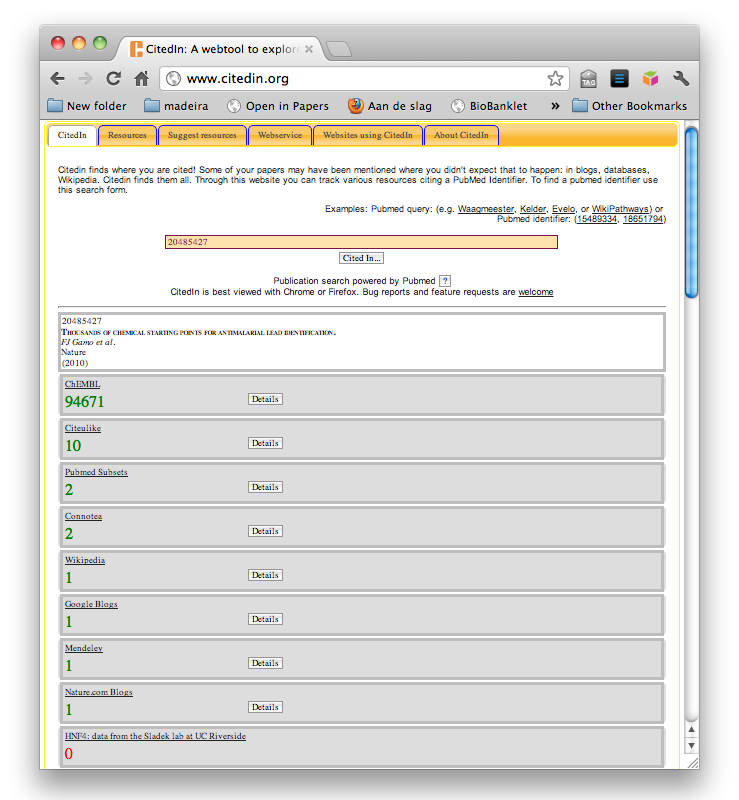
\includegraphics[width=15cm]{citedin.png}
		\caption[wee]{Screenshot of the CitedIn web service showing a paper cited 94671 times in the ChEMBL database.
		   The \textit{Details} button on the webpage links to a ChEMBL webpage with detail on what parts of the database are
		   linked to that paper.}
	\label{fig:citedin}
		\end{center}
\end{figure*}

\begin{figure*}[!ht]
		\begin{center}
		bioclipse-ds.png
		%\includegraphics[width=15cm]{bioclipse-ds.png}
		\caption[wee]{Screenshot from Bioclipse Decision Support with results from a ChemSpider + ChEMBL-RDF search. The top left canvas contains the query structure, in this case the drug Carbamezapine, the top right canvas shows the near neighbors in ChemSpider (via a similarStructure search) that contain ChEMBL-RDF data, the lower right shows the chemical structure for the selected compound in the top right canvas, and the lower left canvas shows the found interactions for this compound using ChEMBL-RDF.}
	\label{fig:bioclipse-ds}
		\end{center}
\end{figure*}

\newpage

\begin{table*}
\caption{Prefixes and their matching namespaces used in this paper.} \label{namespaces}
\begin{center}
\begin{tabular}{ll}
\hline
\multicolumn{2}{l}{\textbf{Common Vocabularies}} \\
bibo    & Bibliography Ontology~\cite{Giasson2011} \\
        & http://purl.org/ontology/bibo/ \\
chebi   & Chemical Entities of Biological Interest~\cite{DeMatos2010} \\
        & http://purl.org/obo/owl/CHEBI\# \\
cheminf & Chemical Information Ontology~\cite{Hastings2011} \\
        & http://semanticscience.org/resource/ \\
cito    & Citation Typing Ontology~\cite{Shotton2010} \\
        & http://purl.org/spar/cito/ \\
obo / pro & OBO \& PRotein Ontology~\cite{Sidhu2006} \\
          & http://purl.obolibrary.org/obo/ \\
bfo     & Basic Formal Ontology~\cite{Smith2004} \\

\multicolumn{2}{l}{\textbf{ChEMBL-RDF Namespace}} \\
chembl & http://rdf.farmbio.uu.se/chembl/onto/\# \\

\multicolumn{2}{l}{\textbf{ChEMBL-RDF Prefixes }}\\
act    & http://linkedchemistry.info/chembl/activity/ \\
assay  & http://linkedchemistry.info/chembl/assay/ \\
mol    & http://linkedchemistry.info/chembl/molecule/ \\
res    & http://linkedchemistry.info/chembl/resource/ \\
\hline
\end{tabular}
\end{center}
\end{table*}


\end{bmcformat}
\end{document}
